\documentclass{article}
\usepackage{v-problem}
\vgeometry

\begin{document}
\vtitle[KINEMATICS]

\def\pn{06}
\def\book{Irodov}
\def\page{14}
\def\question{
Two particles, $1$ and $2$, move with constant velocities $v_1$ and $v_2$ along two mutually perpendicular straight lines toward the intersection point $O$. At the moment $t = 0$ the particles were located at the distances $l_1$ and $l_2$ from the point $O$. How soon will the distance between the particles become the smallest? What is it equal to?
}

\def\option{
}


\vspace*{\fill}
\begin{tikzpicture}
	\node[qnumber] (n) at (0, 0)[scale=2] {$\pn.$};
	\node[question] (q) [right=2mm of n.east] {\question};
	\tzline[divider]<-0.125, 0> (q.north west)(q.south west);
	\node[format] (f) at  (q.south east){[\book \quad \page]};
	%\node[diagram] (d) [below=2cm of q.south] {\diagram};
	%\node[option] (o) [below=1cm of d.south] {\option};
\end{tikzpicture}	
\vspace*{\fill}
\begin{center}
\begin{tikzpicture}
	\tzcoor*(0, 0)(O){$O$}[br]
	
	\tzline+[->, thick]($(O)+(-4, 0)$)(1, 0){$v_1$}[ar]
	\tzline+[dashed](O)(-4, 0)
	\tzdot*($(O)+(-4, 0)$)(5pt)
	\tzline[|<->|]<0, -0.5>(O)($(O)+(-4, 0)$){$l_1$}[midway, below]

	\tzline+[->, thick]($(O)+(0, 4)$)(0, -1){$v_2$}[l]
	\tzline+[dashed](O)(0, 4)
	\tzdot*($(O)+(0, 4)$)(5pt)
	\tzline[|<->|]<0.5, 0>(O)($(O)+(0, 4)$){$l_2$}[midway, right]
\end{tikzpicture}
\end{center}
\vspace*{\fill}
\end{document}
